\chapter{Méthodes agiles}
Une méthode agile est une approche itérative et incrémentale, qui est menée dans un esprit collaboratif avec juste ce qu’il faut de formalisme.\\
Elle génère un produit de haute qualité tout en prenant en compte l’évolution des besoins des clients. Il existe plusieurs méthodes : Scrum (la plus populaire), XP, le lean software développement, etc. et les techniques proposées sont nombreuses.

\section{Valeurs caractéristiques d’un projet agile}
\begin{itemize}[label=\textbullet]
\item Les individus et les interactions plutôt que les processus et les outils
\item Produit qui fonctionne plutôt qu’une documentation exhaustive
\item La collaboration avec le client plutôt que la contractualisation des relations
\item L’acceptation du changement plutôt que la conformité aux plans
\end{itemize}

\section{Les douzes principes d’une méthode agile}
\begin{itemize}[label=\textbullet]
\item Satisfaire le client est la priorité
\item Accueillir les demandes de changement « à bras ouverts »
\item Livrer le plus souvent possible des versions opérationnelles de l’application
\item Assurer une coopération permanente entre Client et Equipe projet
\item Construire des projets autour d’individus motivés
\item Privilégier la conversation en face à face
\item Mesurer l’avancement du projet en termes de fonctionnalités de l’application
\item Faire avancer le projet à un rythme soutenable et constant
\item Porter une attention continue à l’excellence technique et à la conception
\item Favoriser la simplicité
\item Responsabiliser les équipes
\item Ajuster, à intervalles réguliers, son comportement, ses processus pour être plus efficace
\end{itemize}

\section{L’agilité avec Scrum}
Scrum est un processus agile qui nous conduit à produire la plus grande valeur métier dans la durée la plus courte.\\
Scrum nous permet d’inspecter rapidement et régulièrement (toutes les 1 à 4semaines) un produit
(partiel) qui fonctionne.\\
Le métier identifie les exigences et définit leur priorité. Notre équipe s’organise elle-même pour déterminer
la meilleure façon de produire les exigences les plus prioritaires.
\begin{figure}[h!]  
 \centering
    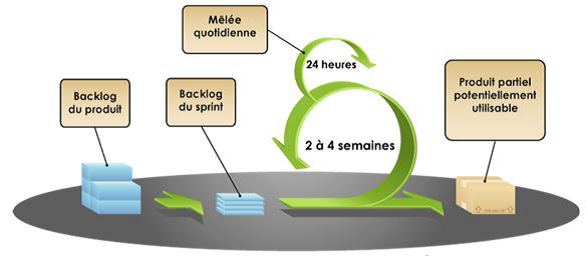
\includegraphics{annexe/Figures/scrum.png}
  \caption{Cycle de vie de la méthode SCRUM}
\end{figure}

Toutes les 1 à 4 semaines, tout le monde peut voir fonctionner le produit actuel et contribuer
à prendre une décision : soit le livrer dans l’état, soit continuer à l’améliorer pendant 2 à 4 semaines
supplémentaires avant de se reposer la question.\\

\subsubsection*{Release}
Pour améliorer la lisibilité du projet, on regroupe généralement des itérations en releases.
Bien que ce concept ne fasse pas explicitement partie de Scrum, il est utilisé pour mieux identifier
les versions. En effet, comme chaque sprint doit aboutir à la livraison d’un produit partiel, un release
permet de marquer la livraison d’une version aboutie, susceptible d’être mise en exploitation.
Il est intéressant de planifier à l’échelle d’un release, en répartissant les items du backlog de produit
sur les sprints, en respectant leur priorité. Bien entendu, ce qui est planifié au-delà du sprint courant
peut changer à tout moment, rien n’est figé à l’avance.\\
\subsubsection*{Sprints}
À la fin du sprint, tout le monde se réunit pour effectuer la revue de sprint, qui dure au maximum 4
heures. L’objectif de la revue de sprint est de valider le logiciel qui a été produit pendant le sprint.
L’équipe commence par énoncer les items du backlog de produit qu’elle a réalisés. Elle effectue ensuite
une démonstration du logiciel produit. C’est sur la base de cette démonstration que le directeur
de produit valide chaque fonctionnalité planifiée pour ce sprint.\\
Une fois le bilan du sprint réalisé, l’équipe et le directeur de produit proposent des aménagements sur
le backlog du produit et sur la planification provisoire de la release. Il est probable qu’à ce moment
des items soient ajoutés, modifiés ou ré-estimés, en conséquence de ce qui a été découvert.